
\chapter{Dimensional Reduction and Visualization Improvements}

Purpose:



\section{Dimensional Reduction}

\subsection{Principal Component Analysis}

Tharrault paper

Russell paper

\section{Meta-Analysis}

\subsection{Out-of-Family Telemetry}

Two NASA papers

\subsection{Out-of-Family Correlations}



\section{Corrgram Enhancements and Dimensional Reduction}

\subsection{Smoothing and Time Adjustments}

\subsection{Ranked Filtering}

\subsection{Fault Filtering}

\subsection{Substring Filtering}

\subsection{Cross-System Filtering}

\subsection{Timelines}


\section{Two-Dimensional Graph Embeddings}

Since the vast majority of user interfaces in common usage are two-dimensional, and hardware limitations can easily result in 3D user interfaces being infeasible for users, it makes sense to look at ways that $n$-dimensional system state data can be embedded within a 2D visualization. Towards this purpose, I did a brief survey of state-of-the-art 2D graph embeddings, looking for implementation feasibility and the ability to give a user ``insight" into the nature of a system fault. Preferably, a 2D embedding for system understanding will make major state transitions and patterns visibly obvious at a glance, and will spatially separate different system ``modes" so that they can easily be mentally grouped by the viewer.

\subsection{Undirected Dependency Graphs}

The first type of two-dimensional graph embedding that we examined as an alternative for animated corrgrams was the ``dependency graph." Dependency graphs are a type of 2D embedding in which a complex system is represented as a directed graph, where nodes are system components and edges represent dependencies; for example, if $\textbf{node}_{A} \rightarrow \textbf{node}_{B}$ and $\textbf{node}_{B} \rightarrow \textbf{node}_{C}$, this indicates that the value of $\textbf{node}_{A}$ depends on the value of $\textbf{node}_{B}$, which in turn depends on $\textbf{node}_{C}$. A simple example of this type of visualization is shown in Fig.~\ref{fig:dependency_graph_example}.

\begin{figure}[h]
\centering
    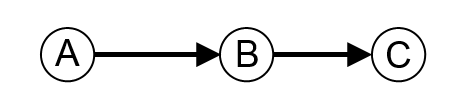
\includegraphics{images/dependency_graph_example.png}
    \caption{A simple example of a traditional dependency graph is shown. Here, node A's value depends on the value of node B, and node B's value depends on the value of node C.}
    \label{fig:dependency_graph_example}
\end{figure}

As such, this type of visualization lends itself well to illustrating the effect of causation in a system. Though causation can be difficult to determine in a complex system, as we have already shown, correlation is calculable via the PCC and other metrics, and a correlation-generalized undirected correlation graph could be envisioned, wherein two nodes have an undirected edge if their mutual PCC score exceeds a certain threshold, and have no edge if their mutual PCC score fails to meet that threshold. The steps to generate such a graph are as follows:

\begin{enumerate}
    \item At a given point in time, generate a PCC matrix for all of the possible data channel pairs.
    \item Generate an unconnected graph in which there exists a degree-0 node for each data channel.
    \item For node-node pair, add a connecting edge if there exists a PCC score above a reasonably high correlation threshold (e.g., $r_{PCC}^{2} > 0.8$). This edge can be colored to show correlation sign (e.g., blue for $r_{PCC} < 0$ and red for $r_{PCC} > 0$).
    \item Finally, cull all nodes that are still of degree 0.
\end{enumerate}

With the corrgram visualization, we needed to illustrate all possible pairs of channels as a separate cell, and thus ended up needing to visualize $\frac{n!}{2 (n - 2)!}$ different cells (where $n$ is the number of data channels). However, with a dependency graph visualization, we can reduce the number of colored elements (nodes) to a count of $n$, by introducing connecting edges. (For systems that are not highly correlated, this will produce far less visual clutter than the corrgram visualization.) Furthermore, we can simplify the undirected dependency graph visualization by eliminating any components of degree 0, if the correlated components are the only ones we wish to see.

We experimented with actually creating this visualization for explorational purposes. First, we ran a system dynamics simulation for our lunar rover described in Chapter 5. We paused the telemetry analysis at a certain time step at which interesting correlated components were present, and examined the data channel correlations at that instant. The correlated components are illustrated in the correlation map visualization in Fig.~\ref{fig:comparison_correlation_map}. We then isolated the correlated components and illustrated them as an undirected dependency graph, using the steps outlined above. The resulting undirected dependency graph visualization, with positive and negative correlation edges both visible, is shown in Fig.~\ref{fig:undirected_both}. In addition, positive and negative correlated components have been isolated into separate graphs for readability and discoverability, as shown in Fig.~\ref{fig:undirected_positive_only} and Fig.~\ref{fig:undirected_negative_only}, respectively.

\begin{figure}[h]
\centering
    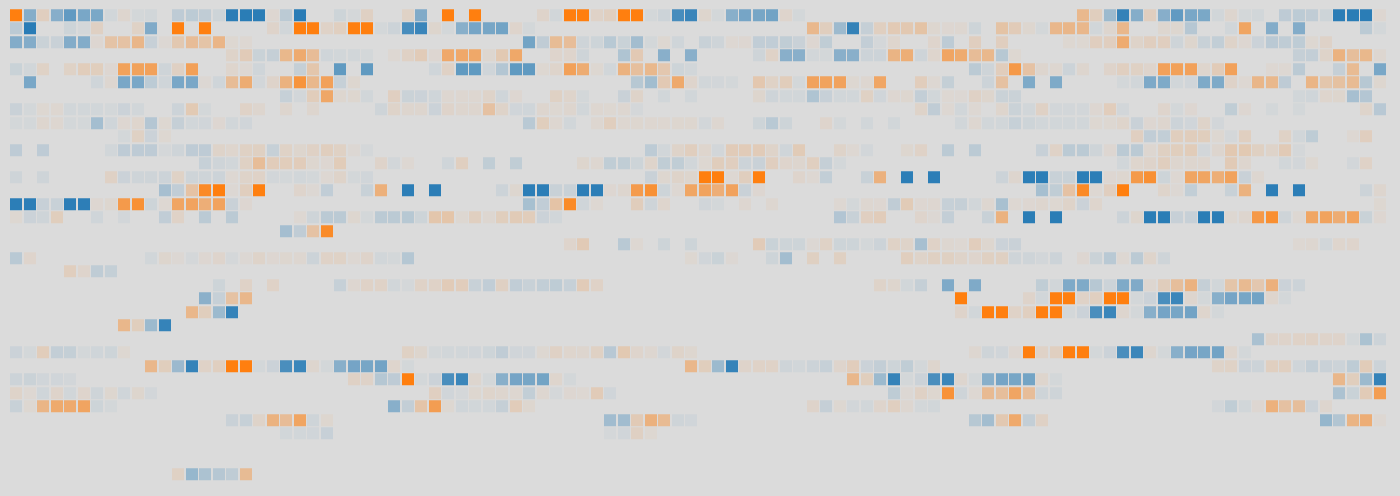
\includegraphics[width=\columnwidth]{images/comparison_correlation_map.png}
    \caption{A snapshot of the correlation map display from a simulated run. Note the strong correlations illustrated by opaque orange (positive) and blue (negative) cells.}
    \label{fig:comparison_correlation_map}
\end{figure}

\begin{figure}[h]
\centering
    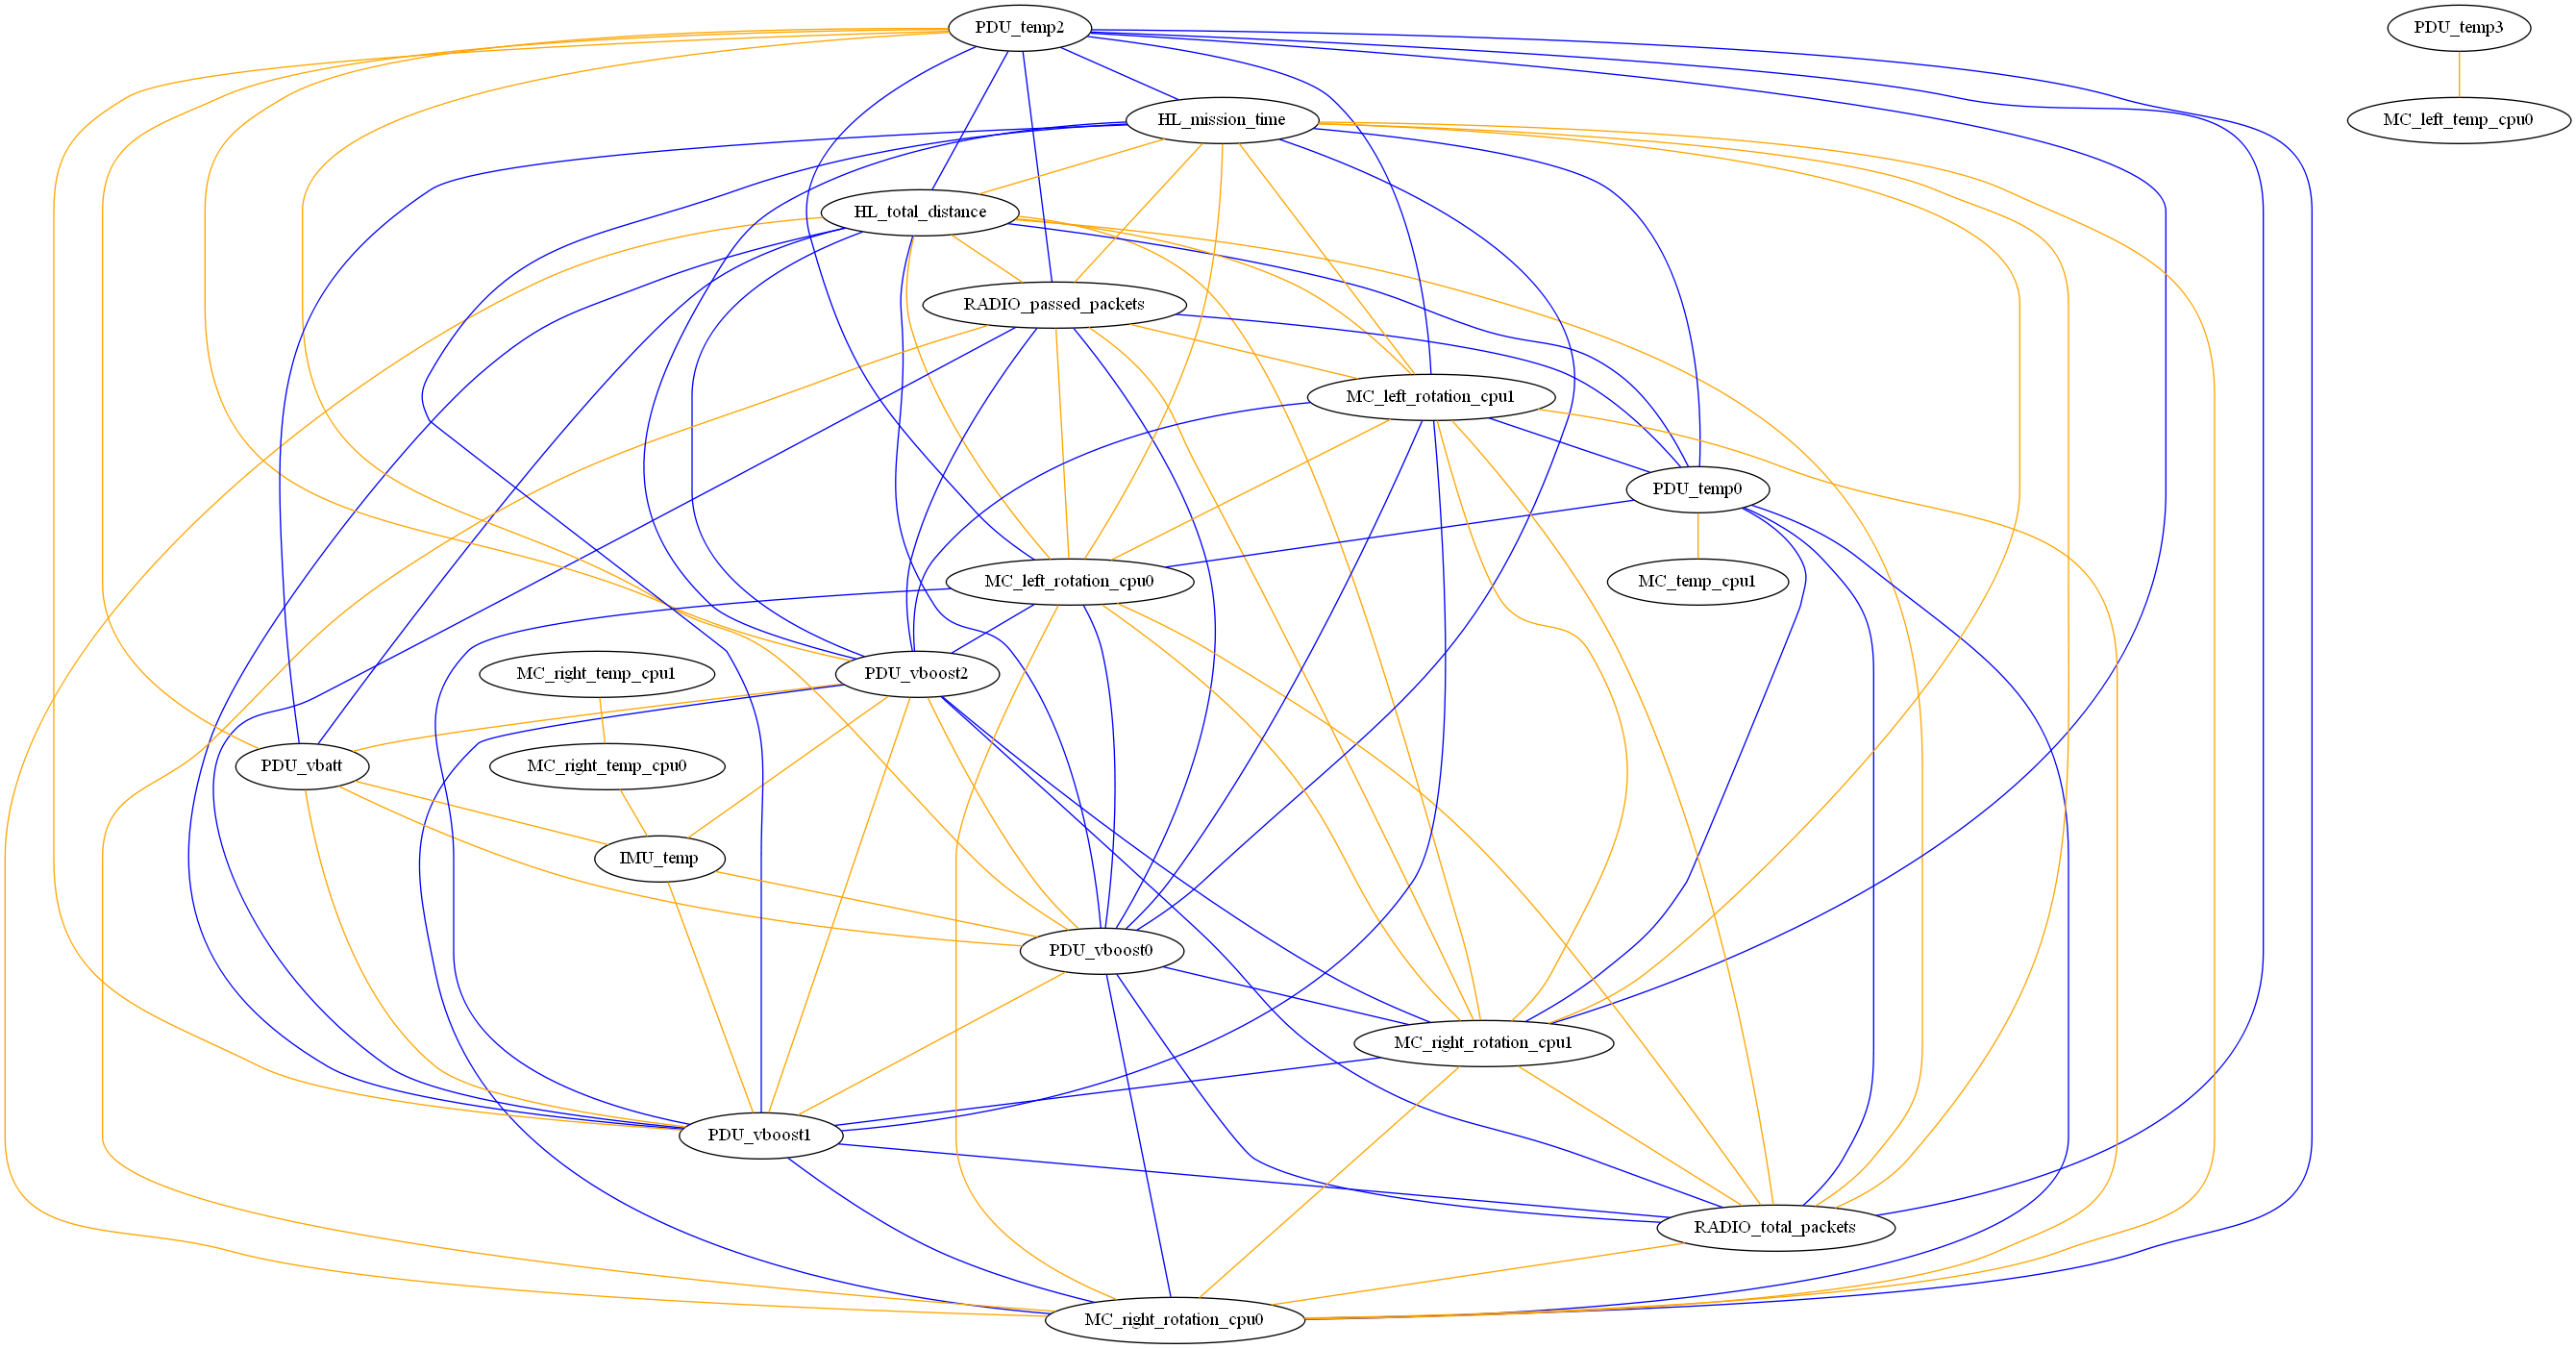
\includegraphics[width=\columnwidth]{images/undirected_both.png}
    \caption{A snapshot of an undirected dependency graph display from a simulated run. Correlated components have been isolated, with edges drawn for all correlation relationships exceeding a certain value ($r_{PCC}^{2} > 0.8$). Both positive and negative correlation connections are shown. Self-correlations are not shown.}
    \label{fig:undirected_both}
\end{figure}

\begin{figure}[h]
\centering
    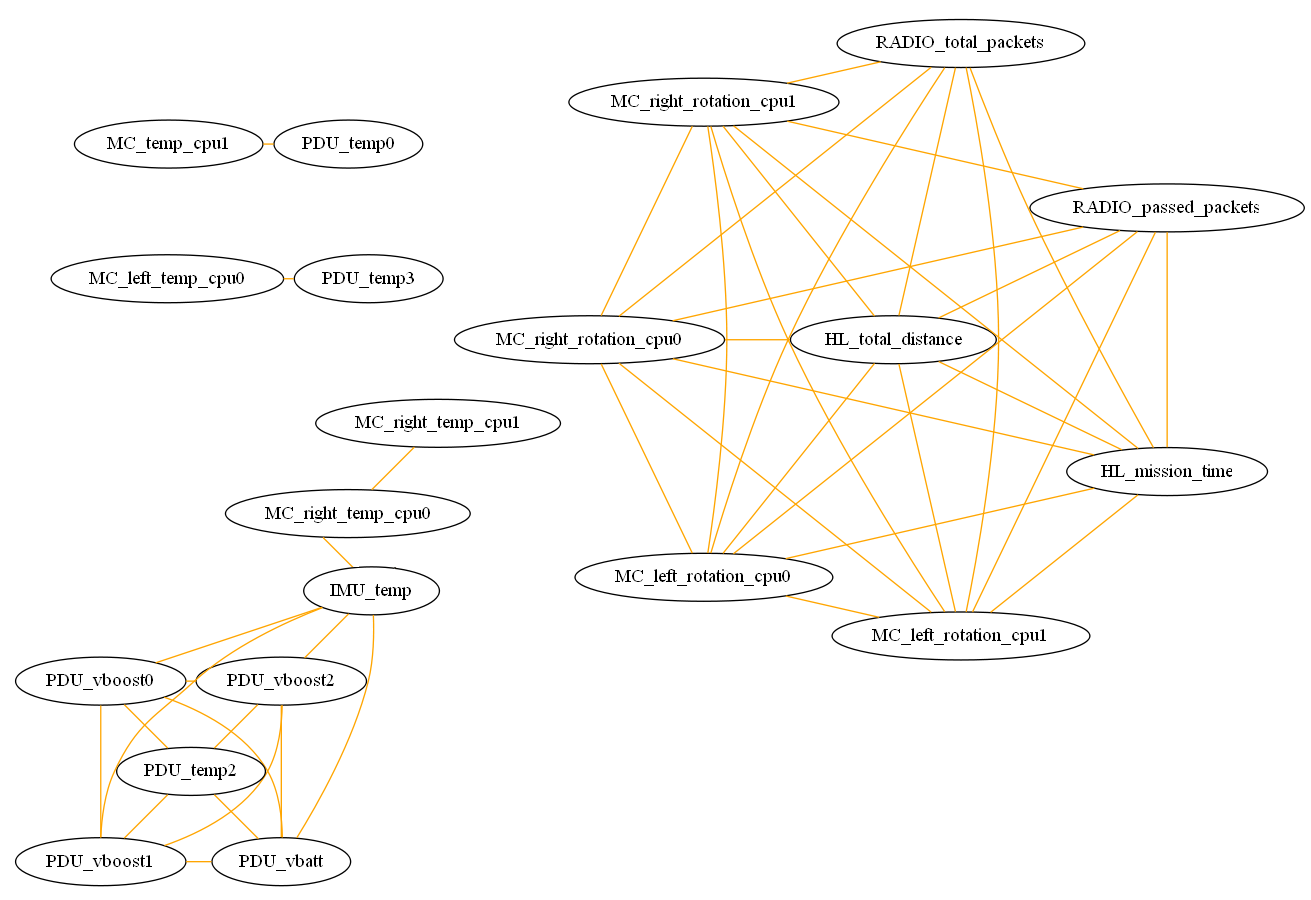
\includegraphics[width=\columnwidth]{images/undirected_positive_only.png}
    \caption{A snapshot of an undirected dependency graph display from a simulated run. Correlated components have been isolated, with edges drawn for all correlation relationships exceeding a certain value ($r_{PCC}^{2} > 0.8$). Only positive correlations are shown. Self-correlations are not shown.}
    \label{fig:undirected_positive_only}
\end{figure}

\begin{figure}[h]
\centering
    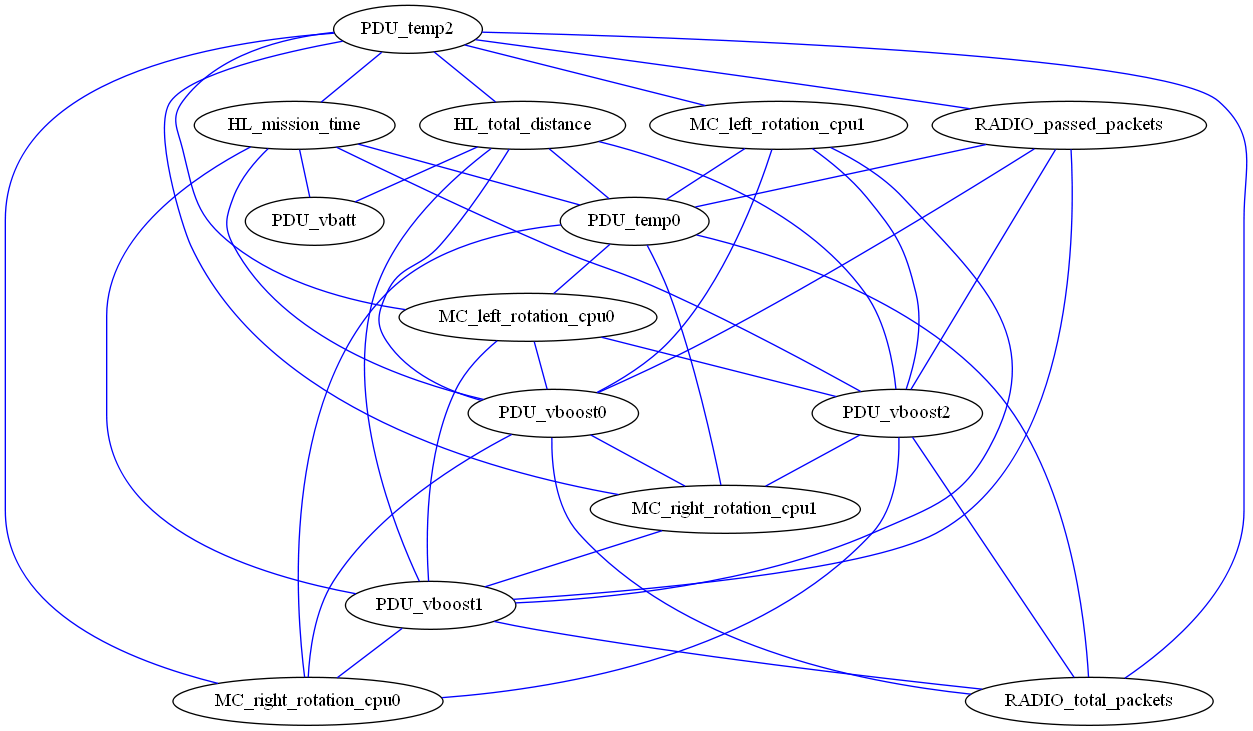
\includegraphics[width=\columnwidth]{images/undirected_negative_only.png}
    \caption{A snapshot of an undirected dependency graph display from a simulated run. Correlated components have been isolated, with edges drawn for all correlation relationships exceeding a certain value ($r_{PCC}^{2} > 0.8$). Only negative correlations are shown. Self-correlations are not shown.}
    \label{fig:undirected_negative_only}
\end{figure}

These visualizations present a very different way of viewing the correlative data. While the temporal dimension is still only captured as a snapshot (i.e., the correlative state at only one time point can be shown at a time), correlated components are shown very clearly, and can be understood at a glance. In particular, the intuition behind the positive correlated components in Fig.~\ref{fig:undirected_positive_only} seems clear; the most fully-connected, major clusters are exhibiting behavior which is very similar to each other. (In fact, the lower left cluster channels were all in a state of monotonic decrease, and the upper right cluster channels were in a state of monotonic increase.) The negative correlated components are less obvious, as they don't ``cluster" in the same way; however, the negative correlation data can be overlaid onto the positive correlation graphs as a higher-level operation on the clusters. This, perhaps, produces the most informative type of graph; this application is shown in Fig.~\ref{fig:undirected_positive_with_negative_clusters}.

\begin{figure}[h]
\centering
    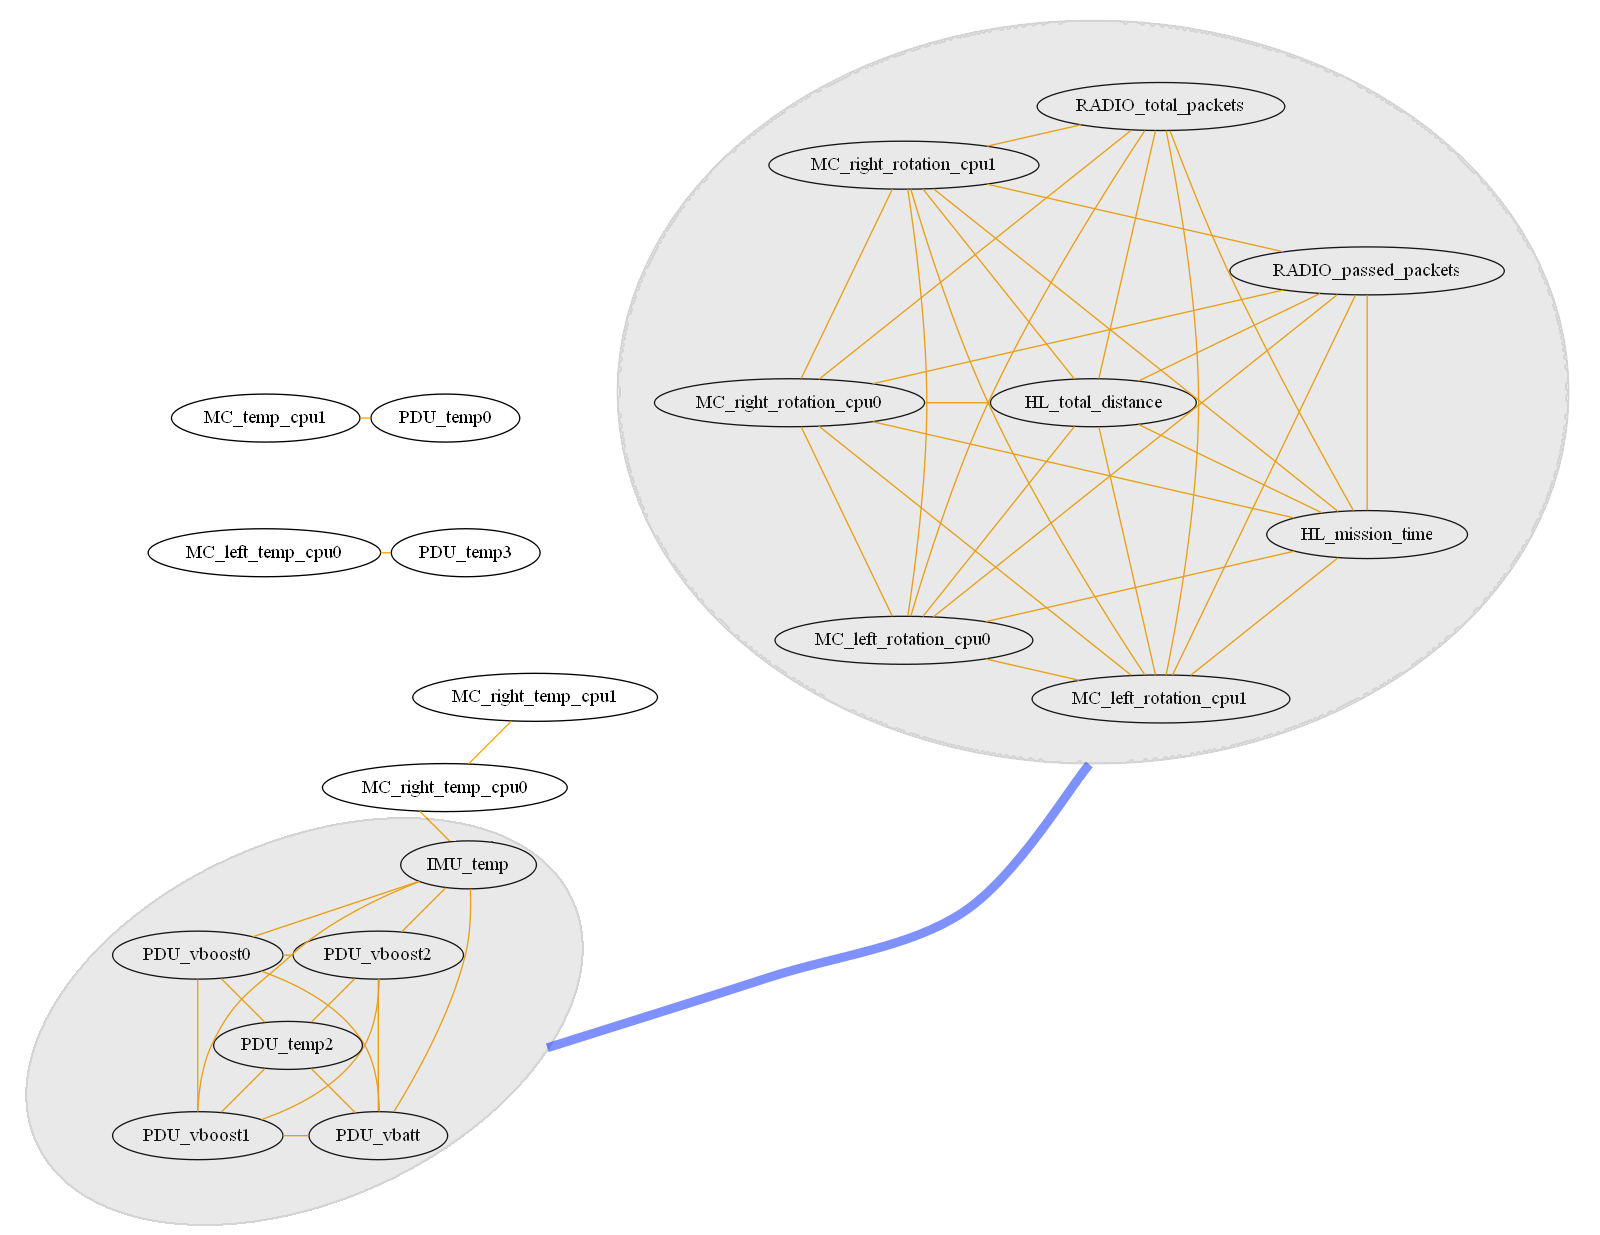
\includegraphics[width=\columnwidth]{images/undirected_positive_with_negative_clusters.png}
    \caption{A snapshot of an undirected dependency graph display from a simulated run. Correlated components have been isolated, with edges drawn for all correlation relationships exceeding a certain value ($r_{PCC}^{2} > 0.8$). Positive correlations, and negatively correlated subgraphs, are shown. Self-correlations are not shown.}
    \label{fig:undirected_positive_with_negative_clusters}
\end{figure}

Another advantage of this technique is that it clearly isolates small groups of correlated components; low-degree subgraphs can point towards noisy data, or towards significant links, but if they are persistent, it seems they may suggest interesting correlations that deviate from the patterns exhibiting by the bulk of the data channels, which tend to correlate due to behavior exhibiting positive and negative monotonicity. However, towards the idea of exploring a visualization which can show the evolution of state and correlative data over time, we will look at another technique in the following section.


\section{Time Curves}

In early 2016, Bach et al presented a powerful new type of visualization tool called ``Time Curves" \cite{bach2016time}. The time curve is a generic 2D embedding algorithm designed specifically for system state data which changes over time. Time curves visualize system states as a series of points, connected in temporal along curves within the 2D embedding. This allows the viewer to gain an understanding of system behavior by the shape and directions of the curves, and by the grouping of the data points. A visual example of how a time curve is ``folded" from an initial linear timeline is shown in Fig.~\ref{fig:time_curve_example}.

\begin{figure}[h]
\centering
    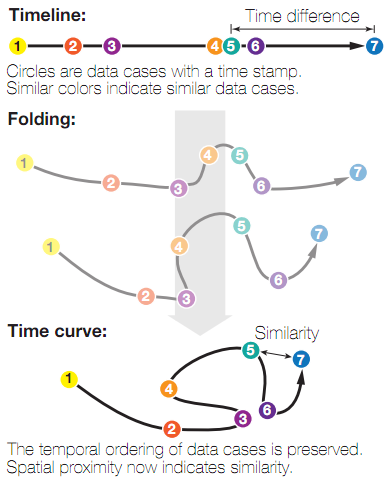
\includegraphics[width=\columnwidth]{images/time_curve_example.png}
    \caption{Three common correlation coefficient algorithms are compared on a sample data set. Note the consistency in visualization for the strong positive correlation between items 1 and 6, and the strong negative correlation between items 4 and 5.}
    \label{fig:time_curve_example}
\end{figure}


\subsection{}

\subsection{}

\subsection{}

\subsection{}



\section{Multidimensional Scaling for Characterizing Correlation Families}

\subsection{}

\subsection{}

\subsection{}

\subsection{}